\documentclass{article}
\usepackage{amsmath}
\usepackage{setspace}
\usepackage{tasks}
\usepackage{graphicx}
\usepackage{listings}

\newcommand{\norm}[1]{\lVert#1\rVert}
\renewcommand{\vec}[1]{\textbf{#1}}
\begin{document}
\onehalfspacing
\begin{center}
  \section*{\textbf{Class 12}}
  \subsection*{Chapter 10 - Vector Algebra}
\end{center}
\begin{enumerate}
  \item If $\theta$ is the angle between and two vectors $\vec{a}$ and $\vec{b}$, then $\norm{\vec{a}^{\top}\vec{b}}$ = $\norm{\vec{a}\times\vec{b}}$ when $\theta$ is equal to
    \begin{tasks}(4)
      \task 0
      \task $\frac{\pi}{4}$
      \task $\frac{\pi}{2}$
      \task $\pi$
      \end{tasks}
\end{enumerate}
  \textbf{Solution:}
  \\
Given,
\begin{align}
  \norm{\vec{a}^{\top}\vec{b}} &= \norm{\vec{a} \times \vec{b}} \label{eq:1}
  \\
  \text{Since, scalar product of two vectors is } \norm{\vec{a}^{\top}\vec{b}} &= \norm{\vec{a}}\norm{\vec{b}}\cos{\theta} \label{eq:2}
  \\
  \text{and vector product of two vector is }\norm{\vec{a} \times \vec{b}} &= \norm{\vec{a}}\norm{\vec{b}}\sin{\theta} \label{eq:3}
\end{align}
Substituting \eqref{eq:3} \eqref{eq:2} in \eqref{eq:1}, we get
\\
\begin{align}
  \implies \norm{\vec{a}}\norm{\vec{b}}\cos{\theta} &= \norm{\vec{a}}\norm{\vec{b}}\sin{\theta}\\
  \implies \cos{\theta} &= \sin{\theta}\\
  \implies \tan{\theta} &= 1\\
  \implies \theta &= \frac{\pi}{4}
\end{align}
\begin{figure}
  \begin{center}
    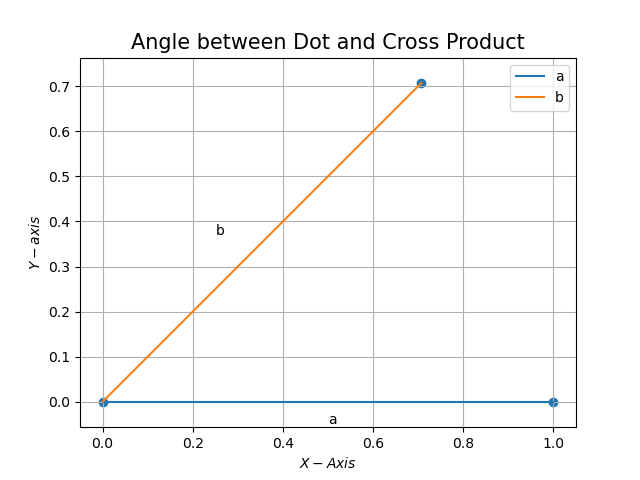
\includegraphics[width=\columnwidth]{/sdcard/Documents/Python/figs/vector.png}
  \end{center}
	\caption{The vectors \vec{a} = 1 and \vec{b} = 1}
  \label{fig:12.10.5.19}
\end{figure}
\end{document}
